\chapter{Validierungsergebnisse der Testszenarien}
\label{cap:Ergebnisse}
Die Architektur des Frameworks besteht somit aus den genannten Modulen, die in
Kapitel~\ref{sec:framework} im Detail beschrieben werden. Ihre
Funktionsweise wird in
Kapitel~\ref{cap:Ergebnisse} anhand von Testszenarien überprüft und ausgewertet.
\section{Überblick und Zielsetzung}

In diesem Kapitel werden die Ergebnisse der im vorherigen Kapitel beschriebenen
Implementierung vorgestellt. Im Fokus steht die Überprüfung der vier
entwickelten Safetymodule – Prozessfolgenüberwachung, Kollisionserkennung,
Achsgeschwindigkeits- und Beschleunigungsüberwachung sowie
Singularitätserkennung – innerhalb der aufgebauten Simulationsumgebung. Ziel ist
es zu überprüfen, inwiefern im gewählten Testsetup eine Detektion von Fehlern in
der Roboterbewegung und Interaktion, welche mit den vier untersuchten Parametern
zusammenhängen, auftreten. Ziel ist es zu überprüfen, inwiefern im gewählten
Testsetup eine Erkennung von Fehlern in der Roboterbewegung und Interaktion,
welche mit den vier untersuchten Parametern zusammenhängen, auftreten.

Für jedes Modul wurden gezielte Testfälle definiert, die sowohl korrekte als
auch fehlerhafte Szenarien abbilden, um die Funktionsweise und Zuverlässigkeit
der Module zu überprüfen. Die Ergebnisse werden anhand von Beobachtungen aus der
Simulation, gespeicherten Zustands- und Ereignisdaten sowie grafischen
Darstellungen aufgezeigt. Die Testfälle wurden dabei als Pfade in RobotStudio
definiert. Diese Pfade werden von RobotStudio in RAPID-Code umgewandelt und
gespeichert. Durch die Synchronisation mit dem Controller und dem Setzen des
aktuellen Programms als Standardprogramm lässt sich das Programm in RobotStudio
simulieren. So wurde für jedes Szenario vorgegangen.

Zur zusätzlichen Validierung wurde ein Experteninterview durchgeführt, in dem
die Testcases vorgestellt und die Funktionsweise des Frameworks diskutiert
wurden. Die Aussagen des Experten werden an geeigneter Stelle in diesem Kapitel
dargestellt und in Kapitel \ref{cap:diskussion} kritisch eingeordnet.

\section{Auswertung der Prozessflussüberwachung}
\label{sec:processauswertung}

Die Validierung der Prozessflussüberwachung erfolgt über die Ausführung eines
korrekten Szenarios als auch eines fehlerhaften Szenarios. Der Fehler soll
provoziert werden, in dem das Werkstück abweichend zum in Abbildung
\ref{figure:Prozessfluss} gezeigten gewünschten Ablauf direkt in das zweite
Regal bewegt wird. Semantisch bedeutet dies ein Überspringen der Station
\textit{Machine}. Das soll ein SafetyEvent triggern, sobald das Werkstück im
falschen Regal abgelegt wird.
\newpage
\textbf{Korrekter Prozessfluss}
\begin{enumerate}
  \item Bewegung von Home-Position zu linkem Regal
  \item Greifen des Werkstücks
  \item Bewegung zu Maschine
  \item Platzieren des Werkstücks in Maschine
  \item Warten auf Beendigung des Bearbeitungsprozesses in
    Warteposition (Bearbeitung hier nur simuliert)
  \item Bewegen zum Werkstück und Greifen aus Maschine
  \item Bewegung zu rechtem Regal
  \item Platzieren des Objekts in rechtem Regal
  \item Rückkehr zur Home-Position
\end{enumerate}

\begin{figure}[H]
  \centering
  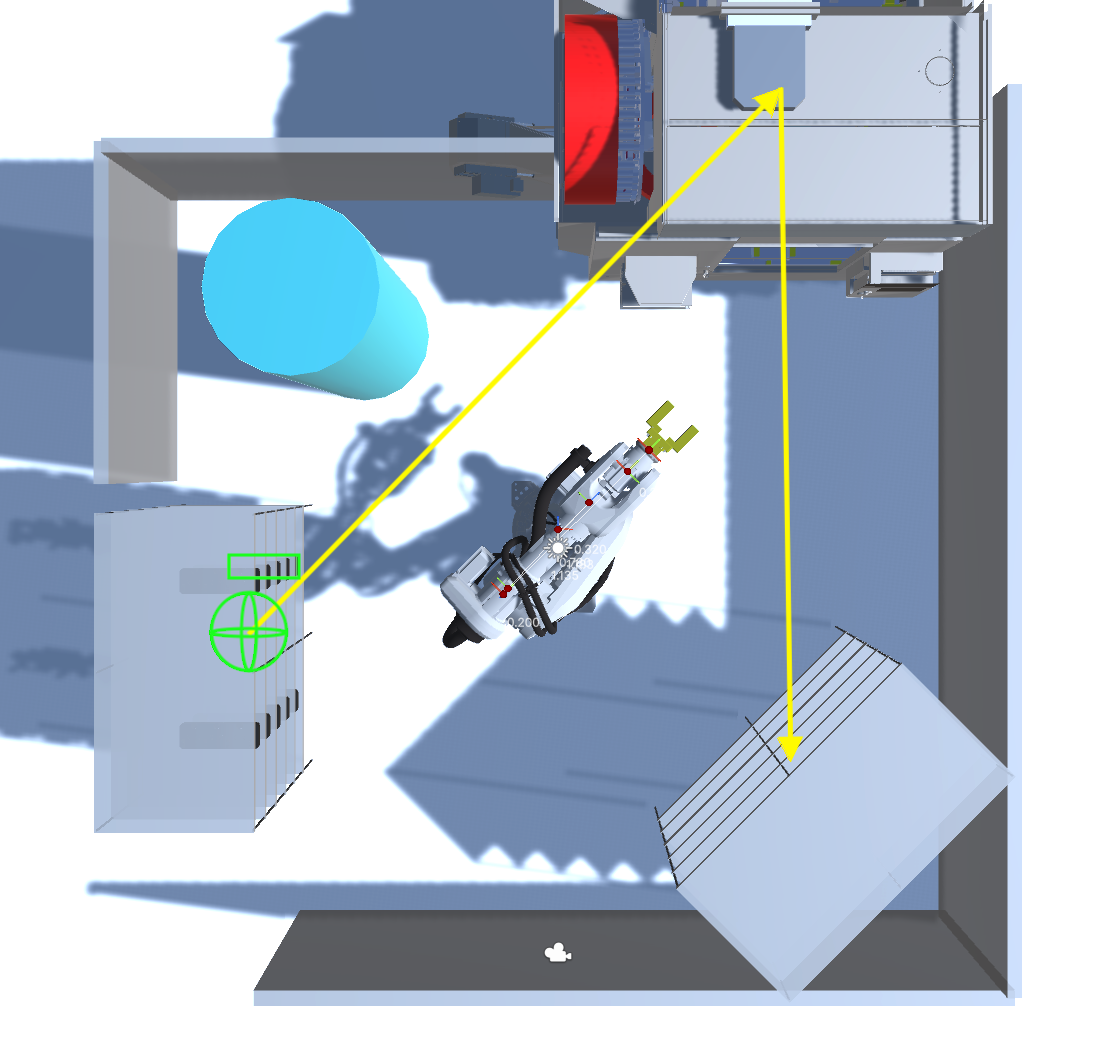
\includegraphics[width=0.7\linewidth]{Figures/Prozessfolge.png}
  \caption{Visuelle Darstellung des Prozessflusses durch Konfiguration der Parts
  und Stations}
  \label{figure:Prozessfluss}
\end{figure}

Im veränderten Prozessfluss wird nun der Schritt der Bearbeitung übersprungen.
Dies kann in der Praxis durch eine inkorrekte Abfolge im Roboterprogrammcode
passieren. Somit ist der veränderte Prozessfluss wie folgt definiert.
\newpage
\textbf{Abgewandelter Prozessfluss}
\begin{enumerate}
  \item Bewegung von Home-Position zu linkem Regal
  \item Greifen des Werkstücks
  \item Bewegung zu Maschine
  \item Bewegung zu rechtem Regal
  \item Platzieren des Objekts in rechtem Regal
  \item Rückkehr zur Home-Position
\end{enumerate}

\subsection{Simulationsergebnis}
Wird der korrekte Prozessfluss durchlaufen, werden in Bezug auf den
ProcessFlowMonitor keine Ereignisse protokolliert.
Bei der Ausführung des Robotercodes mit verändertem Prozessfluss findet sich in
der nach Beendigung des Programms ein JSON-Log, benannt nach
Zeitstempel und Name des Moduls,
welcher einen durch das aufgetretene SafetyEvent des Process Flow Monitors
erstellten Eintrag enthält (vgl. Abbildung~\ref{listing:processflowerror}.)

\begin{figure}[H]
  \inputminted[fontsize=\footnotesize]{json}{code-snippets/processflowerror.json}
  \caption{JSON-Log zum Prozessfolgenfehler, Achswinkel wurden im Nachhinein
  entfernt.}
  \label{listing:processflowerror}
\end{figure}

In Abbildung~\ref{listing:processflowerror} ist abzulesen, dass der
Fehler hier korrekt erkannt und klassifiziert wurde. Dabei zeigt das Feld
\texttt{description} den genauen Hergang des Events an. Hier wurde eine invalide
Transition von StorageIn zu StoraeOut versucht. Das Framework erkennt
ebenfalls, welcher Prozessschritt der Richtige gewesen wäre. Außerdem wird hier
als Violation Type der Type \texttt{SkippedStation} angegeben. Dieser ist als
übersprungene Station zu klassifizieren, was in diesem Fall korrekt ist.
Zusätzlich werden weitere Parameter der Simulation und des Controllers
weitergegeben, unter anderem welches Modul und welche Routine des Moduls zum
Zeitpunkt des Auftretens ausgeführt wurde sowie welcher Programmzeile der
ProgramPointer sich zum Zeitpunkt der Event-Auslösung befand. Durch den Wert des
Keys \texttt{totalSafetyEvents} ist zu erkennen, wie viele Ereignisse bei der
Ausführung vom Programm getriggert wurden. Hier is es lediglich der oben
Genannte.

\section{Auswertung der Kollisionserkennung}
\label{sec:collisionauswertung}

Zur Auswertung der Kollisionserkennung
wurde der oben bereits genannte Prozess genutzt. Anschließend wurde
der Pfad, auf dem sich der Roboter zwischen seiner Home-Position und dem linken
Regal, in dem er ein Werkstück greifen soll, verändert. Rechts dargestellt in
Abbildung \ref{figure:kollision}, führt der Pfad im Gegensatz zum
kollisionsfreien, näher am Roboter verlaufenden Pfad aufgrund des ausladenden
Umschwungs durch die Säulengeometrie. Durch das Abfahren des Pfades gegen den
Uhrzeigersinn wird provoziert, dass der Roboter sich durch die in Abbildung
\ref{figure:kollision} links blau eingefärbte Säule hindurch bewegen
muss. Die Säule ist der Tag \texttt{Obstacle} zugewiesen – sie wird
durch einen vorhandenen Collider,
welcher den Dimensionen der Säule entspricht, zum Kollisionshindernis.

\begin{figure}[!htb]
  \centering
  \begin{minipage}{.535\textwidth}
    \centering
    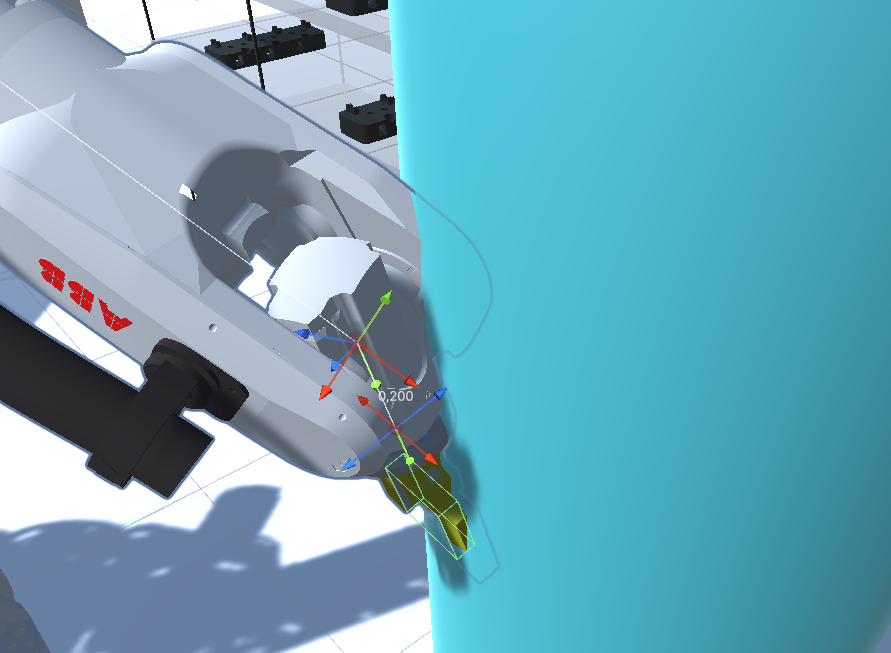
\includegraphics[width=0.9\linewidth]{Figures/CollisionUnity.png}
  \end{minipage}%
  \begin{minipage}{0.465\textwidth}
    \centering
    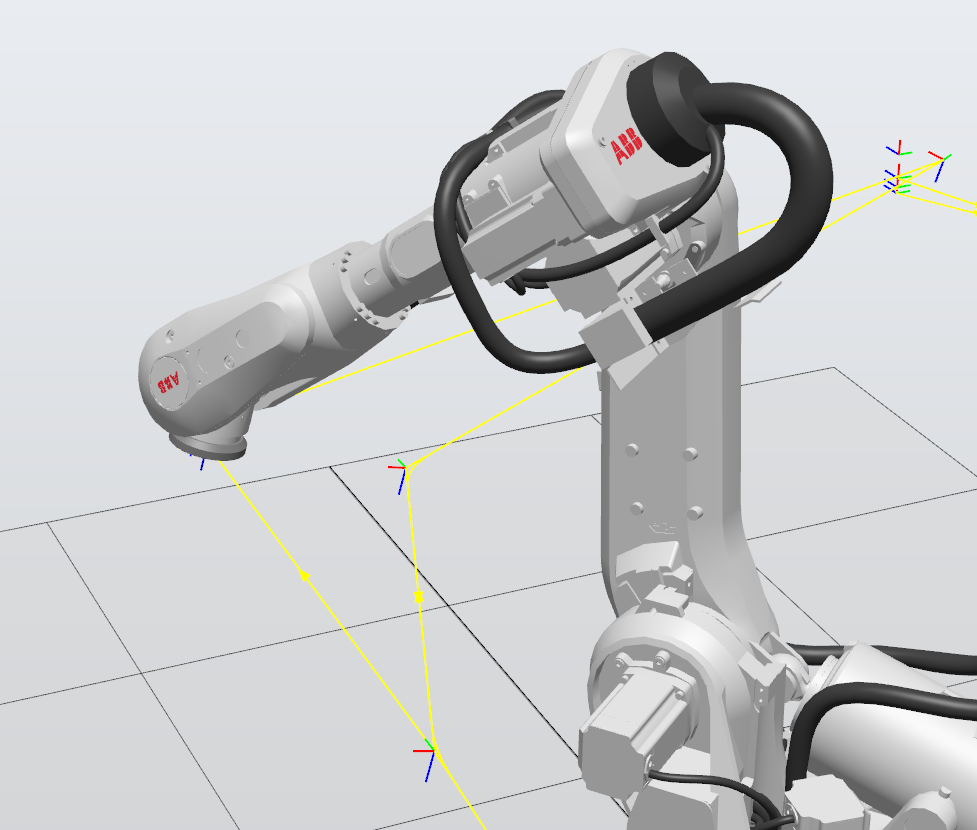
\includegraphics[width=0.9\linewidth]{Figures/CollisionPathRobotStudio.png}
  \end{minipage}
  \caption{Kollision in Unity3D (links) und zugehörige Position auf Pfad in
    RobotStudio (rechts). Gelenk 4, 5 und 6 sowie Greifer befinden
    sich innerhalb der
  Säulengeometrie.}
  \label{figure:kollision}
\end{figure}

\subsection{Simulationsergebnis}

In Abbildung \ref{listing:collisiondetectionerror} ist der Output nach Kollision
mit der Säule dargestellt. Dem Event wurden zusätzlich Eventdaten angefügt,
welche hier den Punkt der Kollision im Unity Koordinatensystem als auch die
Entfernung zum Zentrum des kollidierenden Objekts darstellen. Die Kollision wird
somit zuverlässig erkannt. Wichtig ist dabei zu erwähnen, dass die
Kollisionserkennung stark von den verwendeten Collidern abhängt. Hier verwendet
das Framework Mesh-Collider zur genauen Abbildung der Robotergeometrie, das
Kollisionobjekt wird durch einen primitiven zylindrischen Collider definiert.
Beim Outputformat der eventDataJson handelt es sich um string-escaped JSON. Die
Daten sind also als Event-Daten in einem String komprimiert.\\

\begin{figure}[H]
  \inputminted[fontsize=\footnotesize]{json}{code-snippets/collisiondetection.json}
  \caption{JSON-Log zur Kollisionserkennung. Sich wiederholende
    Key-Value Paare wurden
  verkürzt}
  \label{listing:collisiondetectionerror}
\end{figure}

Weiterführend ist zu erkennen, dass die Kollision mit verschiedenen Gliedern des
Roboters sequentiell erkannt wird. Sobald der Roboter sich visuell weiter in die
Säule bewegt, wird jeweils bei der Kollision mit einem weiteren Glied eine
weitere Kollision erkannt und ein eigenes Event getriggert. Die Reihenfolge der
Joints in diesem Szenario ist nach eingehender Überprüfung als korrekt zu
bewerten, da die Robotergeometrie dafür sorgt, dass Gelenk 4 deutlich breiter
ist als 5 und 6. Gelenk 5 und 6 sind in die Geometrie von Gelenk 4 eingefasst,
daher kollidiert der Roboter initial mit Gelenk 4, bevor eine Kollision an den
kinematisch dahinterliegenden Gelenken erkannt wird.

Zusätzlich dazu lässt sich beim Greifen des Werkstücks feststellen, dass
hier ebenfalls eine Kollision erkannt wird: Durch das Greifen des
Werkstücks wird
eine falsch-positive Kollision getriggert, da bevor das Werkstück gegriffen wird
und semantisch in die kinematische Kette des Roboters verschoben wird, für einen
kurzen Zeitpunkt eine Kollision stattfindet. Ein Beispiel dazu findet sich im
letzten Block von Abbildung \ref{listing:collisiondetectionerror}. Gleiches
lässt sich beim Ablegen des Werkstücks beobachten. Wichtig zu
erwähnen ist der unterschiedlichen Eventtypen, da das Werkstück
aufgrund von fehlendem Tag nicht
als kritisch eingestuft wird.

\newpage
\section{Auswertung der Singularitätserkennung}
\label{sec:singularityauswertung}

Zur Untersuchung der Singularitätserkennung wurde in RobotStudio ein
Szenario erstellt,
das gezielt eine Handgelenks-Singularität provoziert. Dabei wurde der
Roboter in eine Pose
geführt, in der die Achsen~4 und~6 nahezu kollinear verlaufen und
somit die Bedingung
$\theta_{5} \approx 0^\circ$ erfüllt ist. Die Pose ist in Abbildung
\ref{fig:wristSingularity} zu erkennen, hier befindet sich der Roboter nach dem
Greifen des Werkstücks auf dem Weg zum rechten Regal, muss sich für das
Platzieren des Werkstücks im Regal jedoch umorientieren. So kommt die
Singularität
zustande.

\begin{figure}[H]
  \centering
  \includegraphics[width=0.7\textwidth]{figures/wristSingularity.png}
  \caption{Pose in Unity, bei der eine Handgelenks-Singularität mit
  ($\theta_{5} \approx 0^\circ$) entsteht}
  \label{fig:wristSingularity}
\end{figure}

\subsection{Simulationsergebnis}

Die vom Monitor in Unity aufgezeichneten Safety Events sind in
Abbildung~\ref{lst:singularity_json} als gekürzter Auszug
dargestellt. Es werden sowohl
das \enquote{Entering}- als auch das \enquote{Exiting}-Ereignis
erfasst, jeweils mit den
zugehörigen Gelenkwinkeln und einem berechneten
Manipulierbarkeitswert. Nicht relevante
Felder des Snapshots wurden entfernt, da die Gelenkwinkel bereits im
\texttt{eventDataJson} enthalten sind.

\begin{figure}[H]
  \inputminted[fontsize=\footnotesize,breaklines]{json}{code-snippets/singularityerror.json}
  \caption{Gekürzter Auszug der in Unity aufgezeichneten Safety
    Events zur Wrist-Singularität. Zusätzliche Informationen wurden mit "[...]"
  abgekürzt.}
  \label{lst:singularity_json}
\end{figure}

Die Analyse der Ereignisse zeigt, dass der Monitor den Eintritt in
die Wrist-Singularität
bei einer Gelenkkonfiguration von etwa
$[-82.7, -6.9, 36.6, -112.8, -4.9, -153.5]^\circ$ registrierte. Der berechnete
Manipulierbarkeitswert lag hier bei $w \approx 0.19$. Beim Verlassen der Pose
($[-91.8, -8.3, 37.8, -91.3, 5.2, -182.6]^\circ$) wurde das
\enquote{Exiting}-Ereignis
ausgegeben, wobei der Manipulierbarkeitswert mit $w \approx 0.20$
ebenfalls sehr niedrig blieb.
Die Ereignisse decken sich mit dem in RobotStudio provozierten
Szenario und markieren den
Übergang in und aus einer singulären Konfiguration.
Zur Detektion von Singularitäten anderen Typs (hier Schulter- und
Ellbogensingularitäten) wird das gleiche Verfahren angewendet. Hier decken sich
die Ergebnisse mit den oben Beschriebenen.

\section{Auswertung der Gelenkdynamiküberwachung}
\label{sec:Analyse_Sicherheit}
Der Joint Dynamics Monitor erfasst kontinuierlich die Dynamik der sechs
Roboterachsen. Die Implementierung in Unity3D basiert auf den vom digitalen
Abbild gestreamten Gelenkwinkeln, welche aus denen Geschwindigkeiten und
Beschleunigungen differenziell berechnet werden. Zur Signalanalyse werden
mehrere Mechanismen kombiniert, darunter exponentielle Glättung sowie
Fenster-basiertes Mittel zur Dämpfung von Ausreißern. Zusätzlich wird ein
Sicherheitsfaktor von 0{,}8 auf die in RobotStudio spezifizierten Maximalwerte
angewendet, sodass die Schwellwerte im Monitor niedriger liegen als die realen
physikalischen Limits (vgl. Implementierung in
\texttt{JointDynamicsMonitor.cs}). Hier wird mittels des Befehl \texttt{v7000}
im RAPID-Code in RobotStudio die Geschwindigkeit auf den programmierbaren
Maximalwert gesetzt. Dies wurde an zwei Stellen der Roboterbewegung umgesetzt:
Bei der Bewegung von der Home-Position zum linken Regal und bei der Bewegung
nach dem Greifen des Werkstücks zur Maschine. Als primäre Drehachse ist hier
eine Überhöhung der Geschwindigkeit von Gelenk 1 (zentrale horizontale Drehachse
des Roboters) zu erwarten.

\subsection{Simulationsergebnis}
Während der Testsimulation wurden durch den Monitor zwei Überschreitungen der
Geschwindigkeitsgrenzen auf \textbf{Joint 1} registriert. Diese Ereignisse sind
in der aus Unity aufgezeichneten Logdatei dokumentiert. Ein Auszug ist in
Abbildung~\ref{lst:jointdynamics_json} dargestellt. Dort wird jeweils die
Überschreitung der Geschwindigkeit und das nachfolgende
\enquote{resolved}-Ereignis vermerkt, zusammen mit dem aktuellen
Gelenkwinkelzustand des Roboters.

\begin{figure}[H]
  \inputminted[fontsize=\footnotesize,breaklines]{json}{code-snippets/jointdynamicserror.json}
  \caption{Gekürzter Auszug der in Unity aufgezeichneten Safety
  Events des Joint Dynamics Monitor, Ereignis widerholt sich}
  \label{lst:jointdynamics_json}
\end{figure}

Zum Vergleich wurden die Gelenkwinkel aus RobotStudio exportiert und
anhand der berechneten
Achsgeschwindigkeiten ausgewertet. Abbildung~\ref{fig:jointdynamics}
zeigt die Ergebnisse:
Im oberen Diagramm sind die Achswinkel aller sechs Gelenke
dargestellt (J1 hervorgehoben in rot),
darunter die berechneten Geschwindigkeiten mit markierten Schwellwertbereichen.
Die rot eingefärbten Abschnitte kennzeichnen Intervalle, in denen die
aus RobotStudio
exportierten Daten die definierte Grenze von $\pm 50\,^\circ$/s überschreiten.
Die blau markierten Bereiche repräsentieren die durch den Monitor in
Unity ausgegebenen
Safety Events.
Zu erkennen ist eine starke Überschneidung der Bereiche.
Weiterführend zeichnet sich vor allem in der zweiten
Geschwindigkeitsüberschreitung eine Verzögerung beim Ein- und Austritt in den
kritischen Zustand ab. Die Events in Unity werden hier zeitverzögert
weitergegeben.

\begin{figure}[H]
  \centering
  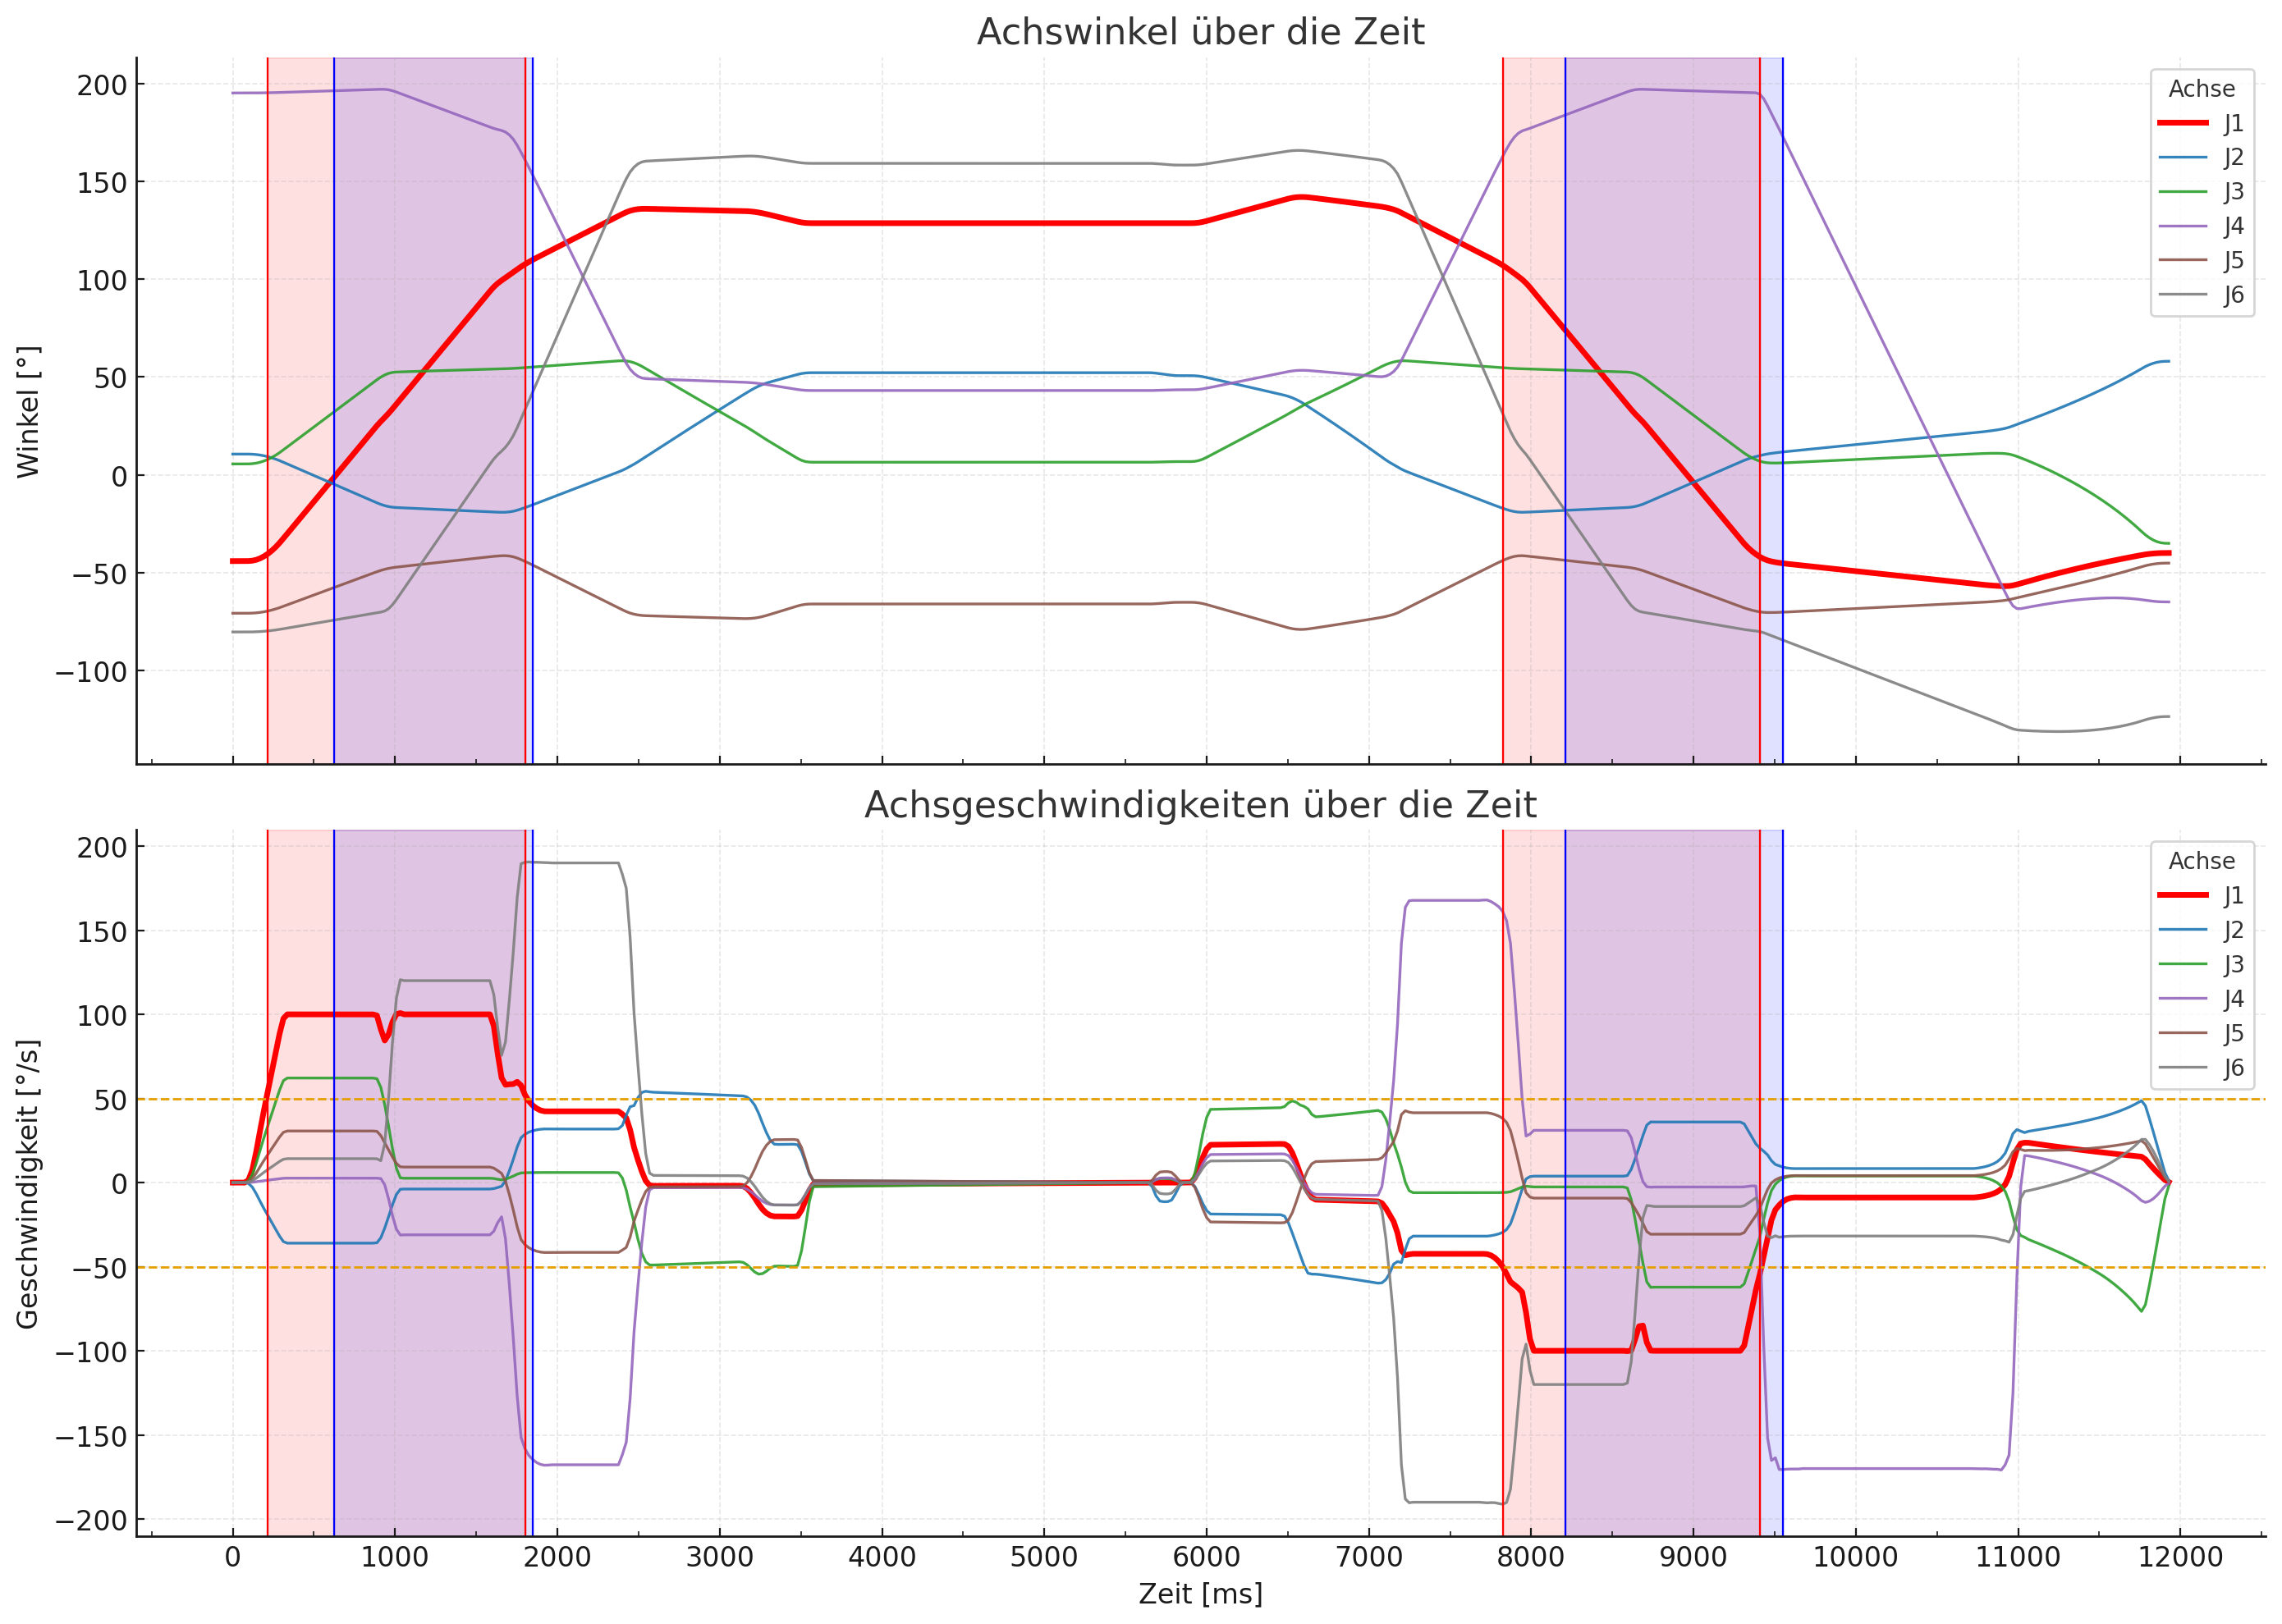
\includegraphics[width=\textwidth]{Figures/achsgeschwindigkeitPlot.png}
  \caption{Achswinkel (oben) und Achsgeschwindigkeiten (unten) mit markierten
    Bereichen (rot: Schwellenübertritte in den Rohdaten, blau: Safety
  Events aus Unity).}
  \label{fig:jointdynamics}
\end{figure}

Eine Gegenüberstellung der Zeitintervalle ist in
Tabelle~\ref{tab:jointdynamics} enthalten.
Dort werden die Start- und Endzeitpunkte der Abschnitte, die Dauer
sowie die Gelenkwinkel
und -geschwindigkeiten an diesen Punkten angegeben. Anhand dieser
Darstellung wird sichtbar,
dass die blau markierten Safety Events zeitlich nach den rot
markierten Schwellenübertritten
liegen. Die in Tabelle~\ref{tab:jointdynamics} und
Abbildung~\ref{fig:jointdynamics} dargestellten Intervalle wurden ermittelt,
indem die aus RobotStudio exportierten Gelenkwinkel mit den in den Safety Events
gespeicherten Zuständen vergleichbar sind. Dazu wurde der euklidische
Abstand zwischen
den Vektoren der Achswinkel berechnet, um den jeweils nächstliegenden
Zeitpunkt in
den Referenzdaten zu bestimmen. Auf diese Weise lassen sich die vom
Monitor in Unity3D
gemeldeten Ereignisse mit den in den Rohdaten beobachteten Schwellenübertritten
korrelieren.

\begin{table}[H]
  \centering
  \small
  \begin{tabularx}{\textwidth}{lrrrrrrX}
    \toprule
    Typ               & Start [ms] & Ende [ms] & Dauer [ms] & Start
    J1 [\textdegree] & Ende J1 [\textdegree] \\
    \midrule
    Dynamik (rot)     & 216        & 1800      & 1584       & -40.35
    & 107.62                \\
    Zielwinkel (blau) & 624        & 1848      & 1224       & -1.25
    & 109.89                \\
    Dynamik (rot)     & 7824       & 9408      & 1584       & 107.08
    & -41.88                \\
    Zielwinkel (blau) & 8208       & 9552      & 1344       & 74.15
    & -45.24                \\
    \bottomrule
  \end{tabularx}
  \caption{Zeitintervalle und Zustände der Joint-Dynamics-Auswertung}
  \label{tab:jointdynamics}
\end{table}

\section{Validierung der Ergebnisse durch Experteninterview}

Im Rahmen der Ergebnisdarstellung wurde ein Experteninterview mit Daniel Syniawa
(M.Sc.) durchgeführt. Ziel war es, die
Funktionsfähigkeit des Frameworks praxisnah zu validieren und Einschätzungen zur
industriellen Einordnung zu gewinnen. Das Interview diente ausschließlich der
\emph{deskriptiven} Ergänzung der Ergebnisse; eine vertiefte Interpretation
erfolgt in Kapitel~\ref{cap:diskussion}.

\subsection{Vorgehen und Gegenstand}

Im Interview wurden die Software und ihre Architektur vorgestellt. Anschließend
wurden die in Kapitel~4 beschriebenen Testfälle gemeinsam in RobotStudio
nachvollzogen: Der Roboter führte die Szenarien aus, während parallel beobachtet
wurde, ob und wie die Module Ereignisse auslösen und ob diese im Logging erfasst
werden. Damit wurde die grundsätzliche Funktionsweise des Frameworks
demonstriert (Auslösen von Safety Events, Erzeugung von JSON-Logs mit
Programmkontext).

\subsection{Beobachtungen}

Prinzipiell konnte ein schnelles Verständnis für die Anwendung des Frameworks
und dessen Funktionsweise gewonnen werden. Bei der Testung der Fälle wurde der
praktische Nutzen der abgespeicherten JSON-Logs hervorgehoben: Für jedes
Ereignis liegen der aktuelle Programmzeiger, das aktuell ausgeführte Programm
sowie die relevante Roboterpose bzw.\ Kontextinformationen vor. Dies erleichtert
die Fehlersuche und macht die Analyse auch für weniger erfahrene Anwender
nachvollziehbar.

\subsection{Hinweis zur Evaluationsmethodik}

Für eine belastbare Evaluation schlug Syniawa vor, die Leistung des Frameworks
\emph{quantitativ} gegen manuelle Verfahren zu vergleichen. Konkret: Wie schnell
findet eine Person den Fehler (z.\,B.\ Auftreten einer Singularität) im
RAPID-Code in RobotStudio im Vergleich zur Erkennung durch Ausführung und
Logging im Framework? Ein solcher Vergleich wäre mit erheblichem Aufwand
verbunden, würde aber die Einordnung der Wirksamkeit deutlich schärfen.

\subsection{Einordnung des Robotersimulations-Ökosystems}

Syniawa wies darauf hin, dass die aktuelle Werkzeuglandschaft stark proprietär
geprägt ist und es nur wenige plattformübergreifende Lösungen mit integrierter
Physik gibt. Häufig ist bereits die stabile Anbindung eines Roboters
herausfordernd; Simulation in RobotStudio erfordert viel Expertenwissen
und Zeit. Die Integration in RWS sei komplex und eher knapp
dokumentiert – insgesamt sei die Nutzerbasis in diesem Bereich klein. Diese
Beobachtungen unterstreichen die Relevanz eines modularen, erweiterbaren
Ansatzes wie in dieser Arbeit umgesetzt.

\subsection{Zusammenfassung}

Das Interview bestätigte die grundsätzliche
Funktionalität des Frameworks in den demonstrierten Testfällen und
identifizierte einen klaren Pfad für eine zukünftige, quantitative Evaluation.
Zudem wurde der praktische Mehrwert der strukturierten Logs (Programmzeiger,
laufendes Programm, Pose/Kontext) betont. Die Einordnung der industriellen
Robotersimulationslandschaft liefert den Rahmen, in dem die
vorgestellten Ergebnisse zu
sehen sind.
\newpage
\section{Zusammenfassung der Ergebnisse}
Die Ergebnisse zeigen, dass die in Unity implementierten Monitore in allen
Testfällen die in RobotStudio provozierten Szenarien widerspiegeln konnten.
Dabei wurde deutlich, dass sich für jedes Modul charakteristische Muster im
Logging abzeichnen: Prozessabweichungen wurden sequenziell dokumentiert,
Kollisionen mit Schweregraden versehen, Singularitäten mit Gelenkwinkeln und
Manipulierbarkeitswerten erfasst, und Geschwindigkeitsverletzungen durch
Event-Paare (exceeded/resolved) gekennzeichnet.

\begin{table}[H]
  \centering
  \small
  \begin{tabularx}{\textwidth}{lXX}
    \toprule
    \textbf{Monitor}      & \textbf{Getestetes Szenario}
    & \textbf{Erkannte Ereignisse / Beobachtungen}
    \\
    \midrule
    Process Flow          & Ablauf mit bewusst fehlerhafter
    Reihenfolge der Operationen                                &
    Abweichung von der erwarteten Sequenz korrekt erkannt, Events
    dokumentieren Verletzung der Prozessfolge.
    \\
    \addlinespace
    Collision Detection   & Simulation mit Kollision zwischen Greifer
    und Werkstück bzw. Störkörper                    & Mehrere
    Kollisionen aufgezeichnet, inklusive beteiligter Objekte; Events
    mit Schweregrad (critical/warning) unterschieden.                 \\
    \addlinespace
    Singularity Detection & Pose in RobotStudio, die eine
    Wrist-Singularität ($\theta_{5} \approx 0^\circ$) provoziert &
    Entering- und Exiting-Events erfasst; Gelenkwinkel und
    Manipulierbarkeitswerte im JSON protokolliert; Szenario deckt
    sich mit RobotStudio. \\
    \addlinespace
    Joint Dynamics        & Bewegung mit Überschreitung der
    Geschwindigkeitsgrenzen auf J1 ($\pm 50^\circ$/s)          & Zwei
    Event-Paare (exceeded/resolved) aufgezeichnet; Verzögerung
    zwischen Schwellenübertritt (Rohdaten) und Event (Monitor)
    sichtbar.       \\
    \bottomrule
  \end{tabularx}
  \caption{Übersicht der getesteten Monitore, Szenarien und erkannten
  Ereignisse im Ergebnisteil}
  \label{tab:monitor_overview}
\end{table}

Die Übersicht in Tabelle~\ref{tab:monitor_overview} verdeutlicht die
Unterschiede
zwischen den Monitoren hinsichtlich Art der Szenarien und Form der
erfassten Events.
Auffällig ist, dass sich in einigen Fällen eine zeitliche Verzögerung zwischen
den in den Rohdaten beobachteten Zuständen und den vom Monitor generierten
Ereignissen zeigt. Diese Beobachtung ergibt sich aus den in Kapitel~3
beschriebenen
Mechanismen (z.\,B. Glättung, Abtastrate).
